\documentclass[10pt,a4paper]{article}
\usepackage[T1]{fontenc}
\usepackage[utf8]{inputenc}
\usepackage[polish]{babel}
\usepackage[margin=2.2cm]{geometry}
\usepackage{amsmath,amssymb}
\usepackage{graphicx,booktabs,enumitem,capt-of}
\setlist{itemsep=1pt,topsep=2pt,parsep=0pt,leftmargin=*}
\setlength{\parindent}{0pt}
\setlength{\parskip}{3pt}
\renewcommand{\arraystretch}{1.12}
\newcommand{\macheps}{\mathrm{macheps}}
\newcommand{\MINsub}{\mathrm{MIN_{sub}}}
\newcommand{\MINnor}{\mathrm{MIN_{nor}}}

\title{}

\begin{document}

\begin{center}
{\Large\bfseries Obliczenia naukowe --- Lista 1: sprawozdanie}\\[3pt]
Krzysztof Zając
\end{center}

Oznaczenia: $t$ --- liczba bitów mantysy (z bitem ukrytym), $u=2^{-t}$ --- precyzja arytmetyki ($\epsilon$ z wykładu), $\delta=2^{-52}$.

%--------------------------------------------------------------------
\section*{Zad. 1 --- macheps, eta, MAX}

\begin{table}[!htbp]
\centering\small
\setlength{\tabcolsep}{4pt}
\begin{tabular}{lrllll}
\toprule
Typ & $t$ & $\macheps$ & $\eta=\MINsub$ & \texttt{floatmin}$=\MINnor$ & MAX \\
\midrule
Float16 & 11 & $2^{-10}\approx 9{,}77\cdot10^{-4}$ & $2^{-24}\approx 5{,}96\cdot10^{-8}$ & $2^{-14}\approx 6{,}10\cdot10^{-5}$ & $65504$ \\
Float32 & 24 & $2^{-23}\approx 1{,}19\cdot10^{-7}$ & $2^{-149}\approx 1{,}40\cdot10^{-45}$ & $2^{-126}\approx 1{,}18\cdot10^{-38}$ & $3{,}40\cdot10^{38}$ \\
Float64 & 53 & $2^{-52}\approx 2{,}22\cdot10^{-16}$ & $2^{-1074}\approx 4{,}94\cdot10^{-324}$ & $2^{-1022}\approx 2{,}23\cdot10^{-308}$ & $1{,}80\cdot10^{308}$ \\
\bottomrule
\end{tabular}
\caption{Wartości wyznaczone iteracyjnie. Są równe wartościom z \texttt{eps}, \texttt{nextfloat(0)}, \texttt{floatmin}, \texttt{floatmax}.}
\end{table}

\begin{itemize}
\item Wartości iteracyjne zgadzają się z \texttt{float.h} dla Float32 (\texttt{FLT\_EPSILON}, \texttt{FLT\_MAX}) i Float64 (\texttt{DBL\_EPSILON}, \texttt{DBL\_MAX}). Float16 nie ma odpowiednika w C.
\item $\macheps=2^{1-t}=2u$. Dla Float64: $\macheps=2^{-52}$, $u=2^{-53}\approx1{,}11\cdot10^{-16}$ (granica błędu względnego zaokrąglenia do najbliższej).
\item $\eta=\texttt{nextfloat(0)}=\MINsub=2^{e_{\min}-t+1}$, $e_{\min}=-14,-126,-1022$.
\item \texttt{floatmin} $=\MINnor=2^{e_{\min}}$ (najmniejsza liczba znormalizowana). $\MINnor/\MINsub=2^{t-1}$ --- tyle jest liczb podnormalnych w każdym typie.
\item $\mathrm{MAX}=(2-2^{1-t})\,2^{e_{\max}}$, $e_{\max}=15,127,1023$. Dla Float16: $65504$.
\end{itemize}

%--------------------------------------------------------------------
\section*{Zad. 2 --- rozmieszczenie liczb Float64}

\begin{minipage}[t]{0.56\linewidth}
\vspace{0pt}
\small
\setlength{\tabcolsep}{3pt}
\begin{tabular}{lll}
\toprule
$x$ & wykładnik (11 b) & mantysa (52 b)\\
\midrule
$0{,}5$ & \texttt{01111111110} & $0\ldots0$\\
$0{,}5+2^{-53}$ & \texttt{01111111110} & $0\ldots01$\\
$1$ & \texttt{01111111111} & $0\ldots0$\\
$1+\delta$ & \texttt{01111111111} & $0\ldots01$\\
$1+2\delta$ & \texttt{01111111111} & $0\ldots010$\\
$2-\delta$ & \texttt{01111111111} & $1\ldots1$\\
$2$ & \texttt{10000000000} & $0\ldots0$\\
$2+2^{-51}$ & \texttt{10000000000} & $0\ldots01$\\
$4$ & \texttt{10000000001} & $0\ldots0$\\
\bottomrule
\end{tabular}
\captionof{table}{\texttt{bitstring} (bit znaku $=0$ pominięty).}
\end{minipage}\hfill
\begin{minipage}[t]{0.42\linewidth}
\vspace{0pt}
\centering
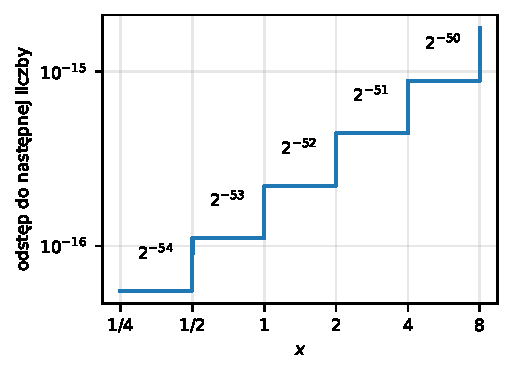
\includegraphics[width=\linewidth]{fig/zad2.pdf}
\captionof{figure}{Odstęp sąsiednich liczb Float64.}
\end{minipage}

\begin{itemize}
\item Test: $10^6$ kolejnych liczb od $1{,}0$ i $10^3$ ostatnich przed $2{,}0$ mają \texttt{nextfloat(x)-x}$=\delta$ i $x=1+k\delta$. Dla $10^5$ losowych $x\in[1,2)$: $k=(x-1)/\delta$ jest całkowite, $1\le k\le2^{52}-1$. Wszystkie testy dały \texttt{true}.
\item W $[1,2)$ wykładnik jest stały, a mantysa to $k$ zapisane binarnie. Przejście $2-\delta\to2$ zwiększa wykładnik.
\item $[\tfrac12,1]$: $x=\tfrac12+k\,\delta/2$, krok $2^{-53}$ (2 razy gęściej).
\item $[2,4]$: $x=2+2k\delta$, krok $2^{-51}$ (2 razy rzadziej).
\item Ogólnie $[2^e,2^{e+1})$: $x=2^e(1+k\delta)$, krok $2^{e-52}$, zawsze $2^{52}$ liczb. Odstęp bezwzględny rośnie z $x$, względny pozostaje w $(2^{-53},2^{-52}]$.
\end{itemize}

%--------------------------------------------------------------------
\section*{Zad. 3 --- $x\cdot(1/x)\neq1$}

\begin{itemize}
\item Skan od \texttt{nextfloat(1.0)} w górę zatrzymuje się na pierwszym kontrprzykładzie, więc (a) i (b) to ta sama liczba:\\
$x=1{,}000000057228997=1+257\,736\,490\cdot2^{-52}$.
\item $\mathrm{fl}\bigl(x\cdot\mathrm{fl}(1/x)\bigr)=0{,}9999999999999999=1-2^{-53}$ (poprzednik $1{,}0$, błąd 1 ulp).
\item Wniosek: dwa zaokrąglenia (dla $1/x$ i dla iloczynu) wystarczą, żeby $x\cdot(1/x)\ne1$. Nie testować odwrotności przez \texttt{==1}.
\end{itemize}

%--------------------------------------------------------------------
\section*{Zad. 4 --- iloczyn skalarny}

\begin{table}[!htbp]
\centering\small
\setlength{\tabcolsep}{5pt}
\begin{tabular}{lrrrr}
\toprule
 & \multicolumn{2}{c}{Float32} & \multicolumn{2}{c}{Float64}\\
\cmidrule(lr){2-3}\cmidrule(lr){4-5}
Metoda & wynik & błąd bezwzgl. & wynik & błąd bezwzgl.\\
\midrule
(a) w przód & $-0{,}49994430$ & $5{,}0\cdot10^{-1}$ & $+1{,}0252\cdot10^{-10}$ & $1{,}1\cdot10^{-10}$\\
(b) w tył & $-0{,}45434570$ & $4{,}5\cdot10^{-1}$ & $-1{,}5643\cdot10^{-10}$ & $1{,}5\cdot10^{-10}$\\
(c) malejąco & $-0{,}5$ & $5{,}0\cdot10^{-1}$ & $0$ & $1{,}0\cdot10^{-11}$\\
(d) rosnąco & $-0{,}5$ & $5{,}0\cdot10^{-1}$ & $0$ & $1{,}0\cdot10^{-11}$\\
\bottomrule
\end{tabular}
\caption{Wartość dokładna: $-1{,}00657107\cdot10^{-11}$.}
\end{table}

\begin{itemize}
\item Żaden wynik nie jest wiarygodny. Float32: błąd $\approx0{,}5$, czyli ok. $10^{10}$ razy więcej niż wynik. Float64: (a), (b) mają błędny znak, (c), (d) dają $0$ (błąd względny 100\%).
\item Przyczyna to uwarunkowanie zadania: $\kappa=\sum|x_iy_i|\,/\,|\sum x_iy_i|\approx5{,}5\cdot10^{17}\gg 1/u=2^{53}\approx9\cdot10^{15}$. Składniki rzędu $\pm2{,}76\cdot10^{6}$ znoszą się do $10^{-11}$.
\item Już same iloczyny w Float64 są zaokrąglone z błędem do $\tfrac12\mathrm{ulp}(2{,}76\cdot10^6)=2^{-32}\approx2{,}3\cdot10^{-10}\gg|\text{wynik}|$. Zmiana kolejności sumowania tego nie naprawia.
\item Kolejność zmienia wynik ((a)$\neq$(b)), ale nie jego jakość. (c) i (d) dają identyczne wyniki w obu precyzjach.
\item Poprawny wynik wymaga wyższej precyzji także dla iloczynów (np. \texttt{BigFloat}).
\end{itemize}

%--------------------------------------------------------------------
\section*{Zad. 5 --- $f(x)=\sqrt{x^2+1}-1$ i $g(x)=x^2/(\sqrt{x^2+1}+1)$}

Błąd względny $\delta$ liczony względem wartości z \texttt{BigFloat} (512 bitów), $x=8^{-k}$.

\begin{table}[!htbp]
\centering\small
\setlength{\tabcolsep}{6pt}
\begin{tabular}{rrllll}
\toprule
$k$ & $x$ & $f(x)$ & $g(x)$ & $\delta_f$ & $\delta_g$\\
\midrule
1 & $1{,}25\cdot10^{-1}$ & $7{,}78222\cdot10^{-3}$ & $7{,}78222\cdot10^{-3}$ & $8{,}4\cdot10^{-15}$ & $7{,}1\cdot10^{-18}$\\
2 & $1{,}56\cdot10^{-2}$ & $1{,}22063\cdot10^{-4}$ & $1{,}22063\cdot10^{-4}$ & $6{,}8\cdot10^{-13}$ & $8{,}3\cdot10^{-17}$\\
3 & $1{,}95\cdot10^{-3}$ & $1{,}90735\cdot10^{-6}$ & $1{,}90735\cdot10^{-6}$ & $1{,}8\cdot10^{-12}$ & $4{,}3\cdot10^{-18}$\\
5 & $3{,}05\cdot10^{-5}$ & $4{,}65661\cdot10^{-10}$ & $4{,}65661\cdot10^{-10}$ & $2{,}3\cdot10^{-10}$ & $1{,}1\cdot10^{-19}$\\
8 & $5{,}96\cdot10^{-8}$ & $1{,}77636\cdot10^{-15}$ & $1{,}77636\cdot10^{-15}$ & $8{,}9\cdot10^{-16}$ & $1{,}6\cdot10^{-30}$\\
9 & $7{,}45\cdot10^{-9}$ & $0$ & $2{,}77556\cdot10^{-17}$ & $1$ & $1{,}4\cdot10^{-17}$\\
10 & $9{,}31\cdot10^{-10}$ & $0$ & $4{,}33681\cdot10^{-19}$ & $1$ & $2{,}2\cdot10^{-19}$\\
\bottomrule
\end{tabular}
\caption{Wybrane wiersze ($k=1,\dots,179$ w pliku wyjściowym).}
\end{table}

\begin{figure}[!htbp]
\centering
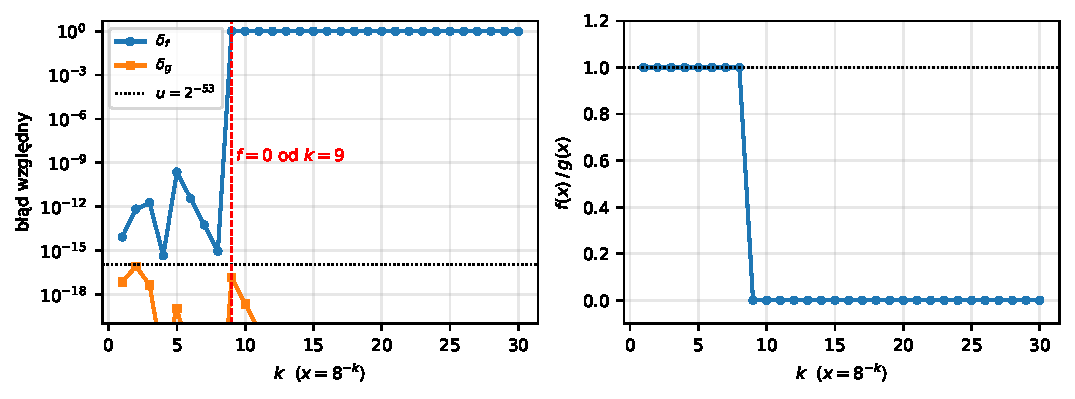
\includegraphics[width=0.92\linewidth]{fig/zad5.pdf}
\caption{Lewy: błąd względny $\delta_f$, $\delta_g$. Prawy: stosunek $f/g$ (powinien być równy 1).}
\end{figure}

\begin{itemize}
\item Wiarygodne jest $g$: $\delta_g\le8{,}3\cdot10^{-17}<u$ dla $k\le178$. Dla $k\ge8$ błąd jest jeszcze mniejszy, bo $\sqrt{x^2+1}+1=2$ i $g=x^2/2$ jest potęgą dwójki (błąd metody $\approx x^2/4$).
\item $f$ jest niewiarygodne. Odejmowanie bliskich liczb ($\sqrt{x^2+1}\approx1$) daje $\delta_f\lesssim u/(x^2/2)\propto64^k$. Błąd rośnie niemonotonicznie ($k=4,8$ trafione szczęśliwie), a to oszacowanie jest górne.
\item Od $k=9$: $x^2=2^{-6k}<2^{-53}$, więc $\mathrm{fl}(1+x^2)=1$ i $f=0$ ($\delta_f=100\%$).
\item $g=0$ dopiero dla $k=179$ (podpływ: $x^2/2\le\MINsub/2$). To limit zakresu, nie algorytmu.
\item Wniosek: przekształcić wzór tak, by uniknąć odejmowania bliskich liczb.
\end{itemize}

%--------------------------------------------------------------------
\section*{Zad. 6 --- pochodna różnicowa $f(x)=\sin x+\cos3x$, $x_0=1$}

Dokładnie: $f'(1)=\cos1-3\sin3=0{,}1169422816885382$. Błąd $E=|f'(x_0)-\tilde f'(x_0)|$, $h=2^{-n}$.

\begin{table}[!htbp]
\centering\small
\setlength{\tabcolsep}{6pt}
\begin{tabular}{rrrrl}
\toprule
$n$ & $h$ & $\tilde f'(x_0)$ & $E$ & $\mathrm{fl}(1+h)$\\
\midrule
0 & $1$ & $2{,}017989$ & $1{,}9$ & $2$\\
10 & $9{,}77\cdot10^{-4}$ & $0{,}120882$ & $3{,}9\cdot10^{-3}$ & $1+2^{-n}$\\
20 & $9{,}54\cdot10^{-7}$ & $0{,}116946$ & $3{,}8\cdot10^{-6}$ & $1+2^{-n}$\\
26 & $1{,}49\cdot10^{-8}$ & $0{,}1169423386$ & $5{,}7\cdot10^{-8}$ & $1+2^{-n}$\\
28 & $3{,}73\cdot10^{-9}$ & $0{,}1169422865$ & $4{,}8\cdot10^{-9}$ & $1+2^{-n}$\\
30 & $9{,}31\cdot10^{-10}$ & $0{,}1169421673$ & $1{,}1\cdot10^{-7}$ & $1+2^{-n}$\\
40 & $9{,}09\cdot10^{-13}$ & $0{,}116821$ & $1{,}2\cdot10^{-4}$ & $1+2^{-n}$\\
50 & $8{,}88\cdot10^{-16}$ & $0$ & $1{,}2\cdot10^{-1}$ & $1+2^{-n}$\\
51 & $4{,}44\cdot10^{-16}$ & $0$ & $1{,}2\cdot10^{-1}$ & $1+2^{-n}$\\
52 & $2{,}22\cdot10^{-16}$ & $-0{,}5$ & $6{,}2\cdot10^{-1}$ & $1+2^{-52}$\\
53 & $1{,}11\cdot10^{-16}$ & $0$ & $1{,}2\cdot10^{-1}$ & $1$\\
54 & $5{,}55\cdot10^{-17}$ & $0$ & $1{,}2\cdot10^{-1}$ & $1$\\
\bottomrule
\end{tabular}
\caption{Wybrane wiersze ($n=0,\dots,54$ w pliku wyjściowym).}
\end{table}

\begin{figure}[!htbp]
\centering
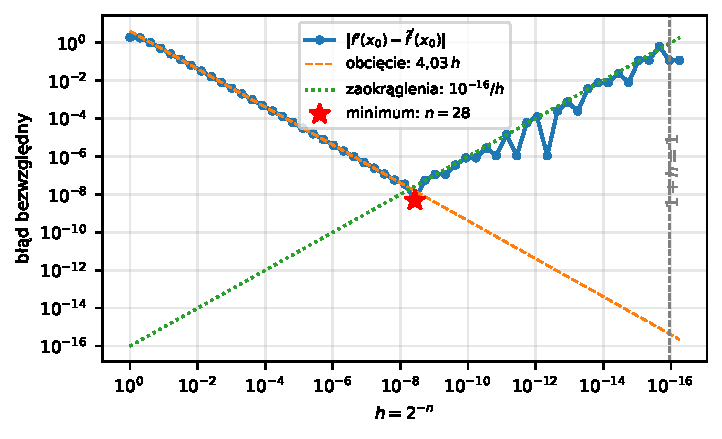
\includegraphics[width=0.72\linewidth]{fig/zad6.pdf}
\caption{Błąd pochodnej w funkcji $h$ (skala log--log).}
\end{figure}

\begin{itemize}
\item $n\le26$: dominuje błąd obcięcia $\approx|f''(x_0)|\,h/2=4{,}03\,h$ ($f''(1)=-\sin1-9\cos3\approx8{,}07$). Przykład: $n=20$, $E=3{,}8\cdot10^{-6}$.
\item Minimum $E$ dla $n=28$ ($h=3{,}7\cdot10^{-9}$, $E=4{,}8\cdot10^{-9}$), rząd $\sqrt{\macheps}\approx1{,}5\cdot10^{-8}$. Sąsiednie $n=27,29$ dają $3{,}5\cdot10^{-8}$ i $5{,}5\cdot10^{-8}$, więc minimum jest częściowo przypadkowe.
\item $n>28$: $E\approx10^{-16}/h$ ($n=30$: $1{,}1\cdot10^{-7}$; $n=40$: $1{,}2\cdot10^{-4}$; $n=45$: $3{,}7\cdot10^{-3}$). To odejmowanie bliskich $f(x_0+h)-f(x_0)$: szum zaokrągleń obliczenia $f$ ($\mathrm{ulp}(\sin x),\mathrm{ulp}(\cos3x)\approx1{,}1\cdot10^{-16}$) dzielony przez $h$. Dalsze zmniejszanie $h$ pogarsza wynik.
\item $1+h$: dla $n\le52$ jest $1+2^{-n}$ dokładnie, więc błąd nie pochodzi z dodawania $x_0+h$. Dla $n\ge53$ jest $h\le u=2^{-53}$ i $\mathrm{fl}(1+h)=1$ (remis do parzystej), licznik $=0$, $\tilde f'=0$, $E=|f'(x_0)|$.
\item $n=50,51$: $1+h\ne1$, ale $\tilde f'=0$. Zmiana $f\approx f'h\approx10^{-16}$ jest rzędu szumu obliczeń $\sin$ i $\cos$, więc $f(x_0+h)=f(x_0)$. Dla $n=52$ licznik wynosi $-2^{-53}$ (zły znak, czysty szum).
\end{itemize}

%--------------------------------------------------------------------
\section*{Wnioski}
\begin{itemize}
\item Pojedyncza operacja ma błąd względny $\le u=2^{-53}$. Problemem jest skracanie przy odejmowaniu bliskich liczb (zad. 4, 5, 6), nie sama arytmetyka.
\item Kolejność działań zmienia wynik (zad. 4), a algebraicznie równoważne wzory dają różną dokładność (zad. 5).
\item Granice zakresu (podnormalne, podpływ, nadmiar) są ostre i przewidywalne (zad. 1, 5).
\end{itemize}

\end{document}